\subsection{Неизмеримые по Лебегу множества}

В прошлый раз была введена мера Лебега, которая определена на $\sigma-$алгебре измеримых подмножеств $\R^n$. Но возникает естественный вопрос: <<Все ли подмножества в $\R^n$ являются измеримыми?>>

Для построения примера не измеримого по Лебегу множества нам понадобится \underline{аксиома выбора.}

\proposition (Аксиома выбора) Пусть задано произвольное семейство абстрактных множеств $\{E_{\alpha} \}_{\alpha \in I}.$ Тогда существует отображение  $F: I \rightarrow \bigcup\limits_{\alpha \in I} E_{\alpha},$ такое что:
$$\forall \alpha \in I \ F(\alpha) \in E_{\alpha}$$\\
Кроме того, корректно определено множество $E = \{F(\alpha) \ | \ \alpha \in I\}.$ 

То есть утверждается, что из любого семейства (не обязательно счетного) множеств можно выбрать по элементу.
\begin{fact}
    Применяя аксиому выбора, мы получаем парадокс Банаха-Тарского: Шар можно разбить на куски, которые можно сложить в два ровно таких же шара. (См Википедию)
\end{fact}

\begin{theorem}
    Для любого измеримого по Лебегу множества $A \subset \R^n$ положительной меры существует его неизмеримое подмножество $E.$
\end{theorem}
\begin{proof}
    Введем в множестве $A$ отношение $\sim:$
    $$x\sim y \Longleftrightarrow x - y \in \Q^n$$
    Ясно, что это отношение эквивалентности (оно рефлексивно, транзитивно, симметрично). Тогда рассмотрим семейство классов эквивалентности $\{E_{\alpha}\}_{\alpha \in I}.$ Пользуясь аксиомой выбора, построим множество $E \subset A.$ $E$ определяется тем, что:
    $$\forall \alpha \in I \ E \cap E_{\alpha} = \{x_{\alpha}\}.$$
    Тогда множество $E$ искомое. Покажем это.\\ Без ограничения общности считаем, что $A$ --- ограничено, то $\exists R > 0: \ ||x - y|| \leq R \ \forall x, y \in A.$ Рассмотрим всевозможные рациональные сдвиги множества $E,$ модуль сдвига которых не превосходит $R.$ По построению:
    $$(E + r) \cap (E + r') = \emptyset, \ r \neq r'$$
    Иначе бы получилось так, что есть в $E$ два элемента, которые лежат в одном классе эквивалентности. С другой стороны:
    $$A \subset \bigcup_{r \in \Q^n, \ ||r|| \leq R} (E + r)$$
    Предположим, что $E$ измеримо, тогда возможны случаи.
    \begin{enumerate}
        \item $\LL^n(E) = 0.$ Но это невозможно, так как $\LL^n(A) > 0.$
        \item $\LL^n(E) > 0.$ Тогда получается, что:
        $$\LL ^n\Bigg(\bigcup_{r \in \Q^n, ||r|| \leq R} (E + r)\Bigg) = \sum_{n = 1}^{+\infty} \LL^n(E + r_n) =  \sum_{n = 1}^{+\infty} \LL^n(E) = +\infty$$
    \end{enumerate}
    Это не возможно, так как $\bigcup\limits_{r \in \Q^n, ||r|| \leq R} (E + r) \in B_{2R}(x) \forall x \in E \Longrightarrow \LL ^n\Bigg(\bigcup_{r \in \Q^n, ||r|| \leq R} (E + r)\Bigg) < + \infty$ 
\end{proof}

\subsection{Регулярность меры Лебега.}

Регулярность по сути означает то, что мы можем <<сложные>> множества приближать более <<простыми>>. Для начала сформулируем следующую теорему:
\begin{theorem}
    (Верхняя регулярность меры Лебега) Пусть $E \subset \R^{n}$ измеримо по Лебегу. Тогда:
    $$\forall \varepsilon > 0 \ \exists \text{ открытое множество }G_{\varepsilon} \text{ такое что }  E \subset G_{\varepsilon} : \ \LL^n(G_{\varepsilon} \setminus E) < \varepsilon$$
\end{theorem}
\begin{proof}
\textbf{Шаг 1.}
    Рассмотрим случай, когда мера $E$ конечна. Тогда по определению верхней меры для любого $\varepsilon > 0$ существует последовательность ячеек $\{P_k\} \subset \PP_n$ такая что: 
    $$\sum_{k = 1}^{\infty} \LL^n(P_k) < \LL^n(E) + \frac{\varepsilon}{2}.$$
    Теперь воспользуемся непрерывность меры слева ($a_k' < a$):
    $$\forall k \in \N \ \forall P_k = [a_k, b_k) \ \exists P'_k = [a'_k, b_k): \ \LL^n(P_k') < \LL^n(P_k) + \frac{\varepsilon}{2^{k + 1}}$$
    $$\forall k \in \N: P_k \subset (a_k', b_k) \subset [a_k', b_k) = P_k'$$
    Тогда определим искомое множество равенством:
    $$G_{\varepsilon} = \bigcup_{k = 1}^{\infty}(a'_k, b_k)$$
    Докажем, что оно подходит, используя счетную полуаддитивность:
    $$\LL^n(G_{\varepsilon}) \leq \sum_{k = 1}^{\infty} \LL^n\Big((a'_k, b_k)\Big) \leq \sum_{k = 1}^{\infty} \LL^n(P_k') \leq \sum_{k = 1}^{\infty} \Big(\LL^n(P_k) + \frac{\varepsilon}{2^{k + 1}}\Big) \leq \LL^n(E) + \frac{\varepsilon}{2} + \frac{\varepsilon}{2}$$
    Кроме того, имеем:
    $$E \subset \bigcup\limits_{k=1}^{\infty}P_k \subset \bigcup_{k = 1}^{\infty}(a'_k, b_k)  \subseteq G_{\varepsilon}$$
    $$\LL^n(G_{\varepsilon} \setminus E) = \LL^n(G_{\varepsilon}) - \LL^n(E) < \varepsilon.$$
    \textbf{Шаг 2.}
    Поскольку $\LL^n$ $\sigma-$конечная мера на $\R^n$, тогда мы можем доказать утверждение для множеств бесконечной меры, <<развалив>> на множества конечной меры. То есть, можно представить множество $E$ в виде дизъюнктного объединения множеств $E_n$ конечной меры. Например, пересекая с кубами с ребром $a$. Понятно что их бесконечное объединение даст искомое множество. Получается:\\
    Если $\LL^n(E) = +\infty$, то:
    $E = \bigsqcup\limits_{k = 1}^{\infty} E_{k}, \text{ т.ч } \forall k \in \N \hookrightarrow \LL^n(E_k) < +\infty. $ \\
    Пользуясь уже доказанным, получим:
    $$\forall k \in \N \ \exists \text{ открытое множество } G_{\varepsilon}(k):\  E_k \subset G_{\varepsilon}(k) \text{ и } \LL^n(G_{\varepsilon}(k) \setminus E_k) < \frac{\varepsilon}{2^k}$$
    Тогда положим $G_{\varepsilon} = \bigcup\limits_{k = 1}^{\infty} G_{\varepsilon}(k).$ Ясно, что $E \subseteq G_{\varepsilon}$ и $G_{\varepsilon}$ открытое. Осталось проверить, что мера их разности меньше $\varepsilon$. Имеем:
    $$G_{\varepsilon} \setminus E = \Big(\bigcup_{k = 1}^{\infty}  G_{\varepsilon}(k)\Big) \setminus E  = \bigcup_{k = 1}^{\infty} \Big( G_{\varepsilon}(k) \setminus E \Big) \subset \bigcup_{k = 1}^{\infty} \Big( G_{\varepsilon}(k) \setminus E_k \Big)$$
    Теперь осталось воспользоваться счетной полуаддитивностью меры Лебега:
    $$\LL^n(G_{\varepsilon} \setminus E) \leq \sum_{k 
 =1}^{\infty}\LL^n\Bigg( G_{\varepsilon}(k) \setminus E_k \Bigg) < \varepsilon$$
\end{proof}

\begin{corollary}
    (регулярность меры Лебега). Пусть $E$ измеримо по Лебегу. Тогда: 
    \begin{enumerate}
        \item  $\LL^n(E) = \text{inf}\{\LL^n(G): \ G - \text{ открытое } E \subseteq G\}$
        \item  $\LL^n(E) = \text{sup}\{\LL^n(F): \ F - \text{ замкнутое } F \subseteq E\}$
        \item  $\LL^n(E) = \text{sup}\{\LL^n(K): \ K - \text{ компакт } K \subseteq 
        E\}$
    \end{enumerate}

\end{corollary}
\begin{proof}
    \textbf{Пункт 1.} Мгновенно следует из предыдущей теоремы. \\
    \textbf{Пункт 2.} Применим предыдущую теорему для $\R^n \setminus E:$
        $$\forall \varepsilon > 0 \ \exists G_{\varepsilon}: \ \R^n \setminus E \subset G_{\varepsilon}, \ \LL^n(G_{\varepsilon} \setminus E) < \varepsilon$$
        Но тогда рассмотрим множество $F_{\varepsilon} = \R^n \setminus G_{\varepsilon}$. Поскольку $E \setminus (F_{\varepsilon}) = G_{\varepsilon} \setminus (\R^n \setminus E)$. Имеем:
        $$\LL^n(E \setminus (F_{\varepsilon})) < \varepsilon$$
        Откуда и вытекает требуемое. \\
    \textbf{Пункт 3.} Для начала поймем, как же нам получить компакт из произвольного замкнутого множества $F$. Заметим, что:
        $$\forall j \in \N: \ K_{j}(F) = F \cap [-j, j]^n - \text{ компакт}$$
        Таким образом, мы построили возрастающую последовательность компактов, поскольку мера Лебега непрерывна снизу, имеем:
        $$\exists \lim_{j\rightarrow \infty}\LL^n(K_{j}(F)) = \LL^n(F) $$
        Согласно предыдущему пункту:
        $$\LL^n(E) = \text{sup}\Big\{\LL^n(F): \ F - \text{ замкнутое } F \subseteq E\Big\} = $$
        $$= \sup\limits_{F \subset E} \sup\limits_{j \in \N} \LL^n(K_j(F)) = \text{sup}\Big\{\LL^n(K): \ K - \text{компакт} \subseteq E\Big\}$$

\end{proof}

\begin{corollary}
    Для любого измеримого $E \subseteq \R^{n}:$
    \begin{enumerate}
        \item Существует возрастающая последовательность компактов $\{K_j\}, \ K_j \subseteq E \ \forall j \in \N:$
        $$E = \bigcup_{j = 1}^{\infty} K_j \cup e,\ \LL^n(e) = 0$$
        \item Существует убывающая последовательность открытых множеств $\{G_j\}, \ E \subseteq G_j $ таких, что$ \forall j \in \N$, кроме того:
        $$ e \cup E = \bigcap_{j = 1}^{\infty} G_j,\ \LL^n(e) = 0$$
    \end{enumerate}
\end{corollary}
\begin{proof}
    Докажем первое, а второе доказывается аналогично. Рассмотрим для начала случай, когда $E$ имеет конечную меру. По доказанному:
    $$\LL^n(E) = \text{sup}\{\LL^n(K): \ K - \text{ компакт } K \subseteq E\}$$
    Тогда существует последовательность компактов $K'_1, K'_2, \dots, K'_j:$
    $$\LL^n(E) = \lim_{k \rightarrow \infty} \LL^n(K'_j)$$
    По этой последовательности построим возрастающую последовательность компактов:
    $$K_j = \bigcup_{k = 1}^{j} K'_j, \ j \in \N.$$
    И при этом:
    $$\LL^n(E) = \lim_{k \rightarrow \infty} \LL^n(K_j).$$
    Значит:
    $$\LL^n(E \setminus K_j) = \LL^n(E) - \LL^n(K_j) \rightarrow 0, \ j \rightarrow \infty.$$
    Теперь осталось показать, что $e := \bigcup\limits_{j = 1}^{\infty} (E \setminus K_j)$ имеет меру нуль. В силу монотонности меры Лебега:
    $$0 \leq \LL^n(e) \leq \LL^n(E \setminus K_j) = \LL^n(E) - \LL^n(K_j) \rightarrow 0.$$
    Откуда получаем требуемое.\\
    Если же $E$ имеет бесконечную меру, то существует: последовательность попарно непересекающихся множеств $E_j$ таких что:
    $\bigsqcup\limits_{j = 1}^{\infty}E_j = E$ и 
    $\LL^n(E_j) < +\infty, \ \forall j \in \N$.\\
    Тогда $\forall j \in \N,$ применив только что доказанное, получим:
    $$E_j = \bigcup_{i = 1}^{\infty}K_{ij} \cup e_j.$$
    Следовательно:
    $$E = \bigsqcup_{j = 1}^{\infty} \left(\bigcup_{ = 1}^{\infty}K_{ij} \cup e_j\right).$$
    Если мы перенумеруем соответствующие множества одним индексом, то можем получить:
    $$E = \bigcup_{j = 1}^{\infty}\widetilde{K_{j}} \cup e$$
    Таким образом, требуемое доказано.
\end{proof} 
\remark Множества, которые можно представить в виде счетного объединения компактов, называются сигма компактными, получается любое измеримое это сигма компактное, с точностью до множества меры ноль.
\subsection{Элементы геометрической теории меры.}

Для начала сформулируем 5B-covering lemma.

\begin{lemma}
    (Витали) Пусть $E \subset \R^n$ произвольное ограниченное множество (не обязательно измеримое), $\mathcal{B} = \{B_{\alpha}\}_{\alpha \in I}$ покрытие $E$ шарами. При этом $\text{sup}\{r(B_{\alpha}) | \ \alpha \in I \} < +\infty.$ Тогда существует такое, не более чем счетное \underline{дизъюнктное} подсемейство $\{B_n\}$, где $N \in \N \cup \{+\infty\}$, что:
    $$E \subset \bigcup_{n = 1}^N 5B_n$$
\end{lemma}

\begin{proof}
     Прежде всего заметим, что из ограниченности множества $E$ и ограниченности радиусов следует, что $\exists R > 0$ такое что:
    $$\bigcup_{\alpha \in I}B_{\alpha} \subset B_{R}(0)$$
    План доказательства: берем какой-то шар достаточно большого радиуса (не меньше чем половина размера самого большого шара $R_k$), далее убираем из семейства все шары которые пересекаются с выбранным нами шаром и получаем новое семейство поменьше $\B_{k+1}$, так берем шары пока можем взять. Опишем этот процесс формально, выберем шары раздутые в $5$ раз и покажем, они действительно покрывают $E$:\\
    \textbf{База индукции:} Изначальное семейство совпадает со всем множеством шаров $\mathcal{B}_1 := \mathcal{B}$.\\
    Положим:
        $$R_1 = \sup\Big\{r(B) | \ B \in \mathcal{B}_1\Big\} < +\infty$$
    Пусть:
        $$B_1 - \text{ произвольный шар из } \mathcal{B}_1, \text{ для которого} \ r(B_1) > \frac{R_1}{2}$$
        Пусть:
        $\B_2 = \{B| \ B\cap B_1 = \emptyset \}$ - те шары которые не пересекаются с выбранным шаром \\
    \textbf{Переход:} предположим, что мы построили семейства $\mathcal{B}_i$ и шары $B_i$ при $i = 1, \dots, j$. Положим:
        $$\mathcal{B}_{j + 1} = \{B \in \mathcal{B}|\  B \text{ не пересекает } \bigsqcup_{i = 1}^{j} B_i\}$$
        Если же $\mathcal{B}_{j + 1}$ оказалось пустым, то заканчиваем построение. В противном случае, продолжаем. Положим:
        $$R_{j + 1} = \sup\{r(B) | \ B \in \mathcal{B}_{j + 1}.\}$$
        Пусть
        $$B_{j + 1} - \text{ произвольный шар из } \mathcal{B}_{j + 1}, \text{ для которого} \  r(B_{j + 1}) > \frac{R_{j + 1}}{2}$$
        Заметим, что семейства включены друг в друга: $\B_1 \supset \B_2 \supset \dots \supset \B_{j}$. По построению радиусы не возрастают: $R_1 \geq R_2 \geq ... \geq R_{j}$. А выбранные шары $\{B_i\}_{i=1}^j$ - дизъюнкты.
    Построение закончено, докажем, что оно искомое.\\ 
    Рассмотрим случай, когда построение закончится на $j + 1$ шаге, то есть $\mathcal{B}_{j + 1} = \emptyset$. В таком случае:
    $$\forall B \in \mathcal{B} \text{ пересекает } \bigsqcup_{i = 1}^{j} B_i$$
    Выберем $i \in \{1, \dots, j + 1\}$ минимально возможным, что $B$ пересекает $B_i.$ Докажем, что $r(B) \leq R_i$. \\
    Действительно, при $i = 1$ это очевидно, ведь $R_1$ это супремум радиусов всех шаров и никакой элемент не больше. А если $i > 1,$ то получается, что $B \in \mathcal{B}_{i}$, так как $i$ был выбран минимально возможным, то так как мы еще не выкинули $B$ из семейства, то радиус шара не больше чем супремум по всем радиусам в семействе, тогда получается $r(B) \leq R_i.$

    \begin{minipage}{\textwidth}
    \flushleft
    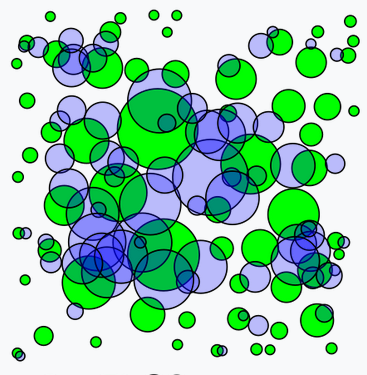
\includegraphics[width=0.45\textwidth]{images/Screenshot_3.png} 
    \flushright
    \vspace{-250pt}
    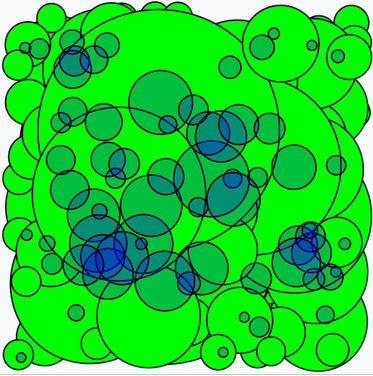
\includegraphics[width=0.45\textwidth]{images/Screenshot_4.png}
    \vspace{10pt}
    \end{minipage}
    \textit{Пояснение к картинке. Мы выбрали зеленые шары. Все остальные синие цепляются как ожерелье за зеленые шары. Мы надуваем зеленые шары в 5 раз и они покрывают все синие шары, а значит и все множество  E} \\
    Теперь зафиксируем точку $x \in E$, так как множество покрыто шарами, то $\exists B: \ x \in B$ пусть центр шара $B_i$ это $x_i,$ а также выберем произвольную точку $y \in B \cap B_i.$ По неравенству треугольника:
    $$||x - x_i|| \leq ||x_i - y|| + ||y - x|| \leq r(B_i) + diam(B) \leq r(B_i) + 2R_i < r(B_i) + 4r(B_i) = 5r(B_i)$$
    Получили, что:
    $$B \subset 5B_i$$
    А отсюда следует требуемое. Ведь $E \subset  \bigcup\limits_{\alpha \in I}B_{\alpha} \subset \bigsqcup\limits_{i = 1}^{j} B_i$

    Теперь же рассмотрим случай, когда построение происходит бесконечно. Получается последовательность попарно непересекающихся шаров $\{B_i\}.$ В силу замечания $\{B_i\} \subset B_{R}(0)$. Поэтому в силу дизъюнктонсти семейства $\{\mathcal{B_i}\}$
    $$\sum_{i = 1}^{\infty} \LL^n(B_i) \leq \LL^n(B_{R}(0)) < +\infty$$
    Мы мажорировали ряд конечным числом, а значит он сходится, но тогда понято что радиусы шаров стремятся к нулю:
    $$\LL^n(B_i) \rightarrow 0, \ j \rightarrow \infty$$
    Следовательно $R_j \rightarrow 0, j\rightarrow \infty$. \\
    Выберем произвольный шар $B \in \mathcal{B}, \ r(B) > 0.$ В силу уже доказанного следует, что $\exists i \in \N : B_i \cap B \neq \emptyset$. Иначе бы $B$ лежал во всех семействах  $\B_i$, но радиус $r(B)$ фиксирован, а радиусы семейств стремятся к $0$. Используя рассуждения аналогичные оценке на радиус шаров в конечном случае, получаем требуемое и в этом случае.
\end{proof}

\begin{definition}
    Пусть $E \subset \R^n$ произвольное множество(даже неизмеримое). Будем говорить, что семейство непустых открытых шаров $\mathcal{B}$ образуют покрытие Витали(fine covering) множества $E,$ если 
    $$\forall x \in E \ \forall r > 0 \ \exists B \in \mathcal{B} \text{ с центром в } x, \text{ таких, что } r(B) < r.$$
    То есть это покрытие множества шарами сколь угодно малого радиуса в каждой точке множества.
\end{definition}

\begin{theorem}
    (Витали о тонком покрытии) Пусть $E \subset \R^n$ произвольное ограниченное множество. Пусть $\mathcal{B} = \{B_{\alpha}\}_{\alpha \in I}$ его покрытие Витали. Тогда существует не более чем счетное \underline{дизъюнктное} подсемейство $\{B_n\}_{n = 1}^N$, где $N \in \N \cup \{+\infty\}$, для которого верно равенство:
    $$\LL^n\Bigg(E \setminus \bigcup_{n = 1}^{N} B_n \Bigg) = 0.$$
\end{theorem}
\remark Предыдущая лемма была грубая в том, что, чтобы покрыть множество нужно было шары раздувать шары в $5$ раз. А это покрытие называется тонким, так как оно покроет множество, но с точностью до меры ноль. Крутость теоремы в том, что из какого-то несчетного набора шаров с какими-то радиусами, из которого можно выделить семейство непересекающихся, таких, что они покроют наше множество с точностью до меры ноль

\begin{proof}
    Выкинем большие шары:
    $$\mathcal{B}_1 = \{B \in \mathcal{B} | \  r(B) \leq 1\}. $$
    Ясно, что семейство образует покрытие Витали множества $E$. Ведь для каждой точки все также есть достаточно малый шар ее покрывающий. Множество $E$ ограничено, радиусы шаров ограничены. Значит к этому семейству $\B_1$ применима лемма Витали. Тогда возможны два случая: \\
    \textbf{Случай 1.} Количество шаров, построенных в лемме Витали конечно. Хотим доказать, что набор который получился $\{B_k\}_{k=1}^{N}$, можно не упятерять, он и так покрывает с точностью до множества меры ноль.\\ Действительно $\mathcal{B}_{N + 1} = \emptyset$ для некоторого натурального $N.$ Любой шар из $\mathcal{B}_1$ пересекает какой-то $B_j.$ \\Ключевой момент(мы хотим это доказать) заключается в том что:
        $$\forall x \in E \setminus (\bigcup_{j = 1}^{N}B_j) \Longleftrightarrow x \in \partial B_j$$
        Действительно, из того что $\mathcal{B}_1$ это покрытие Витали следует, что $\exists \{r_l\}_{l=1}^{\infty}$, стремящаяся к нулю монотонно убывая  $\{B_{r_l}(x)\} \subset \mathcal{B}_1$.
        Значит для некоторого $j \in \N$, а такой $j$ всегда существует, так как шаров конечное число:
        $$\forall l \in \N: \ B_{r_l}(x) \cap B_j \neq \emptyset.$$
        Тогда $x$ - это предельная точка по определению. Тогда мы имеем требуемое. А значит:
        $$E \subset \bigcup_{j = 1}^{N}B_j \cup \bigcup_{j = 1}^{N}\partial B_j$$
        Факт. Границы шаров имеют меру нуль. Так как их конечное количество, то требуемое верно. \\
    \textbf{Случай 2.} Количество шаров бесконечно. То есть $N=+\infty$.\\
    План доказательства и ключевое наблюдение: $\mathcal{B}_{N + 1}$ является покрытием Витали для множества $E_N = E \setminus \left( \bigcup\limits_{i = 1}^{N} \overline{B_i} \right).$ Здесь тонкий момент. Мы покрывали $E$ по построению леммы Витали $N$ шарами. Не покрыли. Значит если точка не попала ни в шар, ни на его границу. То она на положительном расстоянии от этого шара. Тк у нас было fine covering. То существует достаточно малый шар для этой точки, которая никуда не попала. Этот шар лежит в $\B_{N+1}$. Ведь $\B_{N+1}$ не пустое и это по построению семейство шаров, которые ни с кем не пересеклись из выбранных шаров. \\
    Второй еще более тонкий момент. Что происходит дальше. Мы берем этот конечный набор из $N$ шаров. Вычитаем из множества эти шары. Далее у нас остался какой-то обрезанный кусок множества. Для него мы еще раз применяем лемму Витали($C$ это дизъюнктные шары, которые получаются из леммы) Получаем набор шаров $\{C\}$. этот оставшийся кусок множества покрывается $5C$. То есть мы представляем наше множество $E$ как объединение шаров $B$ и Шаров $5C$. А далее мы доказываем, что увеличивая количество $N$ изначально выбранных шаров $B$, то мера $5C$ стремится к нулю. Докажем это формально:
    
    
    Применим лемму Витали для $E_N, \B_{N + 1}:$
        $$E_N \subset \bigcup_{j = N + 1}^{\infty} 5B_j$$
        Но шары не пересекаются, значит действуя по аналогии с предыдущей леммой:
        $$\sum_{j = N + 1}^{\infty}\LL^n(5B_j) \rightarrow 0, N \rightarrow \infty$$
        Тогда:
        $$\LL^n\Bigg(E \setminus \bigcup_{j =1}^{\infty} \overline{B_j}\Bigg) \leq \LL^n\Bigg(E \setminus \bigcup_{j =1}^{N} \overline{B_j}\Bigg) \leq 5^n \sum_{j = N + 1}^{\infty}\LL^n(5B_j)$$
        Отсюда предельным переходом в неравенстве:
        $$\LL^n\Bigg(E \setminus \bigcup_{j =1}^{\infty} \overline{B_j}\Bigg) = 0.$$
        Но используя определение границы:
        $$\LL^n\Bigg(E \setminus \bigcup_{j =1}^{\infty} B_j\Bigg) \leq \LL^n\Bigg(E \setminus \bigcup_{j =1}^{\infty} \overline{B_j}\Bigg) + \LL^n\Bigg( \bigcup_{j =1}^{\infty} \partial B_j \Bigg).$$
        
        Следовательно, так как мера границ шаров равна нулю, их счетное объединение тоже имеет меру ноль, то мы доказали что, хотели
\end{proof}
\begin{note}
    Лемма Витали, и теорема Витали останутся в силе, если требование открытых шаров заменить требованием замкнутых шаров с положительными радиусами (если радиус равен нулю, очевидно нельзя покрыть отрезок такими шарами).
\end{note}

\subsection{Точки плотности}

\begin{minipage}{0.5\textwidth}% adapt widths of minipages to your needs
    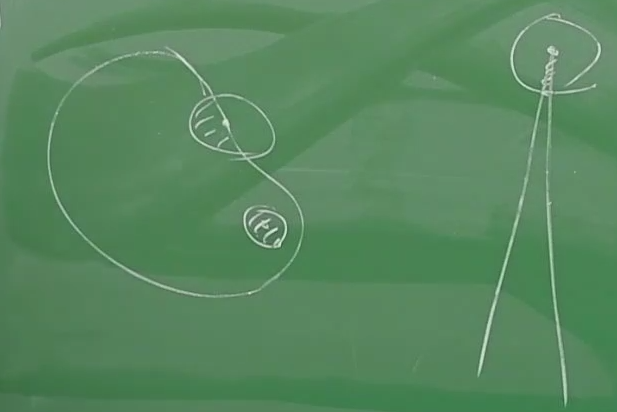
\includegraphics[width=0.8\textwidth]{images/Screenshot_6.png} 
\end{minipage}%
\hfill%
\begin{minipage}{0.5\textwidth}\raggedright
Геометрическая интуиция про точки плотности примерно следующая: берем точку, а в ней шары все меньшего радиуса, и смотрим какая доля шара пересекается с множеством. Верхние примеры, когда шар только частично пересекает множество, а нижний шар полностью лежит в множестве. Так вот теорема о точках плотности как раз про то, что несущественно пересекающих точек <<мало>> (их мера ноль).
\end{minipage}

    \begin{minipage}{\textwidth}


    \end{minipage}

\begin{definition}
    Для точки $x \in E$ определим нижняя плотность равенством $$\underline{D}_{E}(x) = 
    \lowlim_{r \to +0}{\frac{\mu^{*}(E \cap B(x, r))}{\LL^n(B(x, r))}},$$ 
    Кроме того определим верхнюю плотность равенством:
    $$\overline{D}_{E}(x) =\uplim_{r \to +0}{\frac{\mu^{*}(E \cap B(x, r))}{\LL^n(B(x, r))}}$$
\end{definition}
\begin{definition}
    Если $\underline{D}_{E}(x) = \overline{D}_{E}(x) = D_{E}(x)$, то это число называется плотностью точки $x$ относительно множества $E$
\end{definition}
\begin{definition}
    Если $D_{E}(x) = 1$, то $x$ называется точкой плотности множества $E$, то есть:
    
    $$ \exists \lim\limits_{r\ra +0}\frac{\mu^{*}(E \cap B(x, r))}{\LL^n(B(x, r))} = 1.$$
\end{definition}


\begin{theorem}
    Пусть $E \subset \R^n$ --- измеримое по Лебегу множество. Тогда $\LL^n-$ почти всякая точка $x \in E$ является точкой его плотности, то есть:$$\forall \LL^n-\text{почти любая } x \in E \hookrightarrow \exists \lim_{r\rightarrow+0}\frac{\LL^{n}(E \cap B(x, r))}{\LL^n(B(x, r))} = 1.$$
\end{theorem}
\remark В определении плотности в числителе $\mu^*$, так как само множество $E$ не обязательно измеримо, а вот в теореме мы требуем измеримость, поэтому там стоит $\LL^n$.
\begin{proof}
    Зафиксируем $q \in (0, 1)$ и определим множество $E(q)$ равенством:
    $$E(q) = \{ x \in E : \underline{D}_{E}(x) \leq q \}$$
    Значит:
    $$\forall x \in E(q) \ \exists \{r_j(x)\} \text{ последовательность монотонно убывающая к нулю, причем }$$
    $$ \exists \lim_{j \to \infty} \frac{\LL^{n}(E \cap B_{r_j}(x))}{\LL^n(B_{r_j}(x))} \leq q.$$
    Заметим, что
    $$\bigcup_{x \in E_q} \{B_{r_j}(x)\}_{j=0}^\infty  \text{ образует покрытие Витали }E(q)$$
    
    Зафиксируем теперь $\varepsilon \in (0, 1 - q),$ далее будем предполагать, что (иначе можно такие шары <<выкинуть>>, сохранив покрытие Витали):
     $$\frac{\LL^{n}(E \cap B_{r_j}(x))}{\LL^n(B_{r_j}(x))} \leq q + \varepsilon, \ \forall j \in \N.$$
     В силу теоремы Витали, существует дизъюнктный набор шаров $\{B_j(q)\}_{j = 1}^{\infty},$ покрывающий $E(q)$ с точностью до меры $0,$ то есть:
     $$E(q) = \bigcup_{j=1}^{+\infty} B_j(q) \cup e(q), \text{ где } \LL^n(e(q)) = 0$$
     Тогда в силу счетной полуаддитивности меры Лебега:
     $$\LL^n(E(q)) \leq \sum_{j  = 1}^{\infty}\LL^n(E(q) \cap B_j(q)) + \LL^n(e(q)) \leq \sum_{j = 1}^{\infty}(q + \varepsilon) \LL^n(B_j(q)) = (q + \varepsilon)\LL^n(\bigcup_{j = 1}^{\infty}B_j(q)) \leq (*)$$
     Пусть $G$ открытое множество, содержащее $E(q),$ и такое что, $\LL^n(G(q)\setminus E(q)) < \varepsilon \cdot \LL^n(E(q)).$ И далее можем считать, шары содержатся в этом множестве, теперь продолжим оценку:
     $$(*)\leq (q + \varepsilon) \LL^n(G(q)) \leq (q + \varepsilon)(1 + \varepsilon)\LL^n(E(q))$$
     Так как $\varepsilon > 0$ был выбран произвольно, то $\LL^n(E(q)) = 0.$ Тогда $\underline{E} = \{x \in E: \underline{D}_{E}(x) < 1\} \subset \bigcup\limits_{j = 1}^{\infty}E(1 - \frac{1}{2j})$ имеет меру нуль, значит почти все точки $E$ являются точками плотности
\end{proof}